\documentclass[border=2pt]{standalone}
\usepackage[T1]{fontenc}
\usepackage{lmodern}
\usepackage{amsmath}
\usepackage{pgfplots}
\pgfplotsset{compat=1.18}

% ---- brand palette ----
\definecolor{ink}{HTML}{2A2620}
\definecolor{inkfaint}{HTML}{7A6F62}
\definecolor{violet}{HTML}{5A1BA6}
\definecolor{terracotta}{HTML}{A03A2C}
\definecolor{sage}{HTML}{8AA08A}

\begin{document}
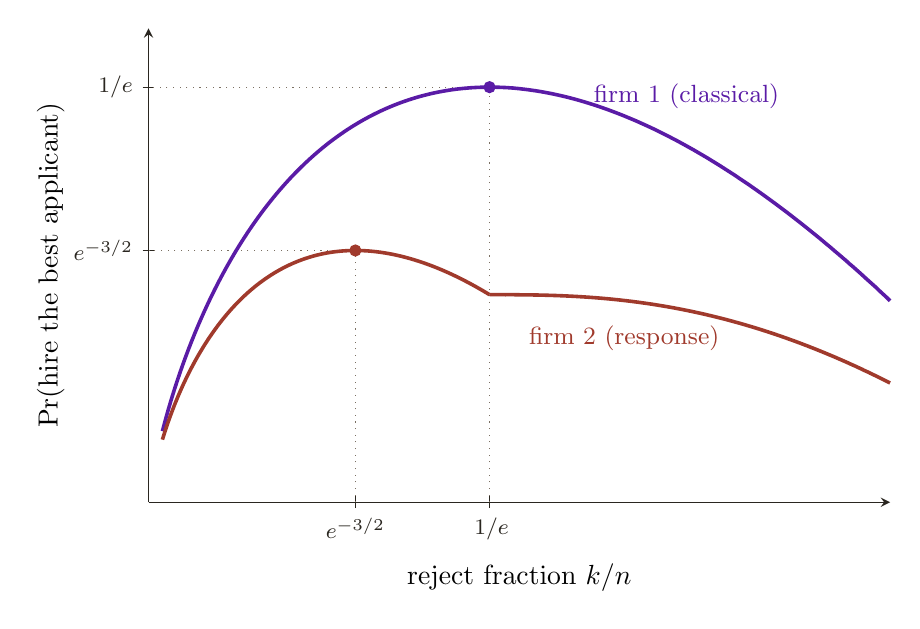
\begin{tikzpicture}
\begin{axis}[
  width=11cm, height=7.6cm,
  axis lines=left,
  axis line style={ink, line width=0.5pt},
  tick style={ink, thin},
  label style={ink, font=\small},
  tick label style={ink, font=\footnotesize},
  every axis x label/.style={at={(axis description cs:0.5,-0.11)},anchor=north},
  every axis y label/.style={at={(axis description cs:-0.1,0.5)},rotate=90,anchor=south},
  xlabel={reject fraction $k/n$},
  ylabel={$\Pr(\text{hire the best applicant})$},
  xmin=0, xmax=0.8, ymin=0, ymax=0.42,
  xtick={0.22313,0.36788}, xticklabels={$e^{-3/2}$,\,$1/e$},
  ytick={0.22313,0.36788}, yticklabels={$e^{-3/2}$,$1/e$},
  clip=false,
]

% guide lines to the two optima
\draw[inkfaint, dotted, thin] (axis cs:0.36788,0) -- (axis cs:0.36788,0.36788) -- (axis cs:0,0.36788);
\draw[inkfaint, dotted, thin] (axis cs:0.22313,0) -- (axis cs:0.22313,0.22313) -- (axis cs:0,0.22313);

% firm 1 (classical): -c ln c
\addplot[violet, line width=1.3pt, samples=250, domain=0.015:0.8] {-x*ln(x)};

% firm 2 best response, branch A (c <= 1/e): -c ln c - c/2
\addplot[terracotta, line width=1.3pt, samples=200, domain=0.015:0.36788] {-x*ln(x)-x/2};
% firm 2 best response, branch B (c > 1/e)
\addplot[terracotta, line width=1.3pt, samples=200, domain=0.36788:0.8]
  {-(x-0.3678794412)*ln(x) + 0.1839397206*(ln(x))^2};

% optima
\addplot[only marks, mark=*, violet, mark size=2pt] coordinates {(0.36788,0.36788)};
\addplot[only marks, mark=*, terracotta, mark size=2pt] coordinates {(0.22313,0.22313)};

% curve labels
\node[violet, font=\small, anchor=west] at (axis cs:0.47,0.36) {firm 1 (classical)};
\node[terracotta, font=\small, anchor=west] at (axis cs:0.40,0.145) {firm 2 (response)};
\end{axis}
\end{tikzpicture}
\end{document}